% Created 2022-09-14 Wed 19:50
% Intended LaTeX compiler: pdflatex
\documentclass[a4paper, 12pt]{article}
\usepackage[utf8]{inputenc}
\usepackage[T1]{fontenc}
\usepackage{graphicx}
\usepackage{longtable}
\usepackage{wrapfig}
\usepackage{rotating}
\usepackage[normalem]{ulem}
\usepackage{amsmath}
\usepackage{amssymb}
\usepackage{capt-of}
\usepackage{hyperref}
\usepackage{geometry}
\geometry{a4paper,margin=30mm}
\usepackage{txfonts}
\usepackage{mathptmx}
\usepackage{hyperref}
\hypersetup{colorlinks=true, citecolor=black, linkcolor=black, urlcolor=blue}
\usepackage{fancyhdr}
\pagestyle{fancy}
\fancyhead[RO,LE]{REMC for Protein Folding}
\usepackage{lastpage}
\fancyfoot[c]{\textbf{Page \thepage/\pageref{LastPage}}}
\author{Paul Etheimer}
\date{\today}
\title{Replica Exchange Monte Carlo Algorithm for protein folding in 2D\\\medskip
\large Programmation 3 et Gestion de projets}
\hypersetup{
 pdfauthor={Paul Etheimer},
 pdftitle={Replica Exchange Monte Carlo Algorithm for protein folding in 2D},
 pdfkeywords={},
 pdfsubject={},
 pdfcreator={Emacs 28.1 (Org mode 9.6)}, 
 pdflang={English}}
\usepackage{biblatex}

\begin{document}

\maketitle
\section*{Introduction}
\label{sec:orga5f84ee}
Monte Carlo algorithms are non-deterministic procedure that use a part of chance to arrive at an answer. They are regularly used for complex problem too hard to solve deterministically, for instance because they have a high degree of freedom. They are particularly useful in the case of optimization, along with other stochastic algorithms such as ant colony optimization or genetic algorithms.


The folding of proteins is such a case of optimization, with many degrees of freedom, involving many physiochemical parameters impossible to properly simulate. One can make several simplifications to reduce the number of parameters, for instance the hydrophobic-polar protein folding model assumes that amino acid broadly belong to two categories, hydrophobic or polar. This simplification rests on the idea that the hydrophobic effect is a driving force of the folding of proteins. It states that solvable, often globular proteins, tend to hide their hydrophobic residues from the environment by grouping them together in a hydrophic core, thus stabilizing the whole protein. The polar amino acid are rather found on the periphery, for instance making hydrogen bonds with the solvent.

The aim of this project is to use a Monte Carlo approach to fold protein in 2D space. We will use a particular kind of Monte Carlo algorithms : the Replica Exchange Monte Carlo algorithm (also called parallel tempering). This kind of Monte Carlo algorithms aims to improve the properties of the standard Markov Chain Monte Carlo, by running several versions of the search (called replicas) at different \emph{temperatures} (a multiplying factor in the decision to accept a change : basically, the higher the temperature, the more likely a negative change is to be accepted). The more favorable replicas, with the lower energy, iterate with the lower temperature, and are more stable, whereas the more the least favorable replicas, with the higher energy, end up with the higher temperature and are more unstable.
\section*{Materials and Methods}
\label{sec:org1d93d46}
The program we have written in \texttt{Python} (3.10), with as sole module used \texttt{numpy} (1.22). The choice of language was imposed, but with as few dependencies, and given the object-oriented nature of our code, a better choice would have been C++. Even though it is not strictly necessary, considering the few dependencies, we have used Docker (actually \texttt{podman}, the RedHat drop-in replacement) to provide a reproducible way to use our program. An alternative, involving cloning the repository and generating the environment with \texttt{conda}, is also available.

The main paradigm used for the development is object-oriented programming. The code consists of three classes, \texttt{AminoAcid}, \texttt{Conformation} and \texttt{Move} \ref{fig:cls} (Appendices). Three additional functions are used, one to run the Monte Carlo search and another to add the replica exchange, and a last one to parse the sequence input. The lattice the conformations evolve in are represented in memory, and copied into the Move instances in order for them to be performed without altering the current conformation.

We only implemented the VSHD neighbourhood (figure \ref{fig:moves}) search, i.e. no \emph{pull moves}. With only \emph{end}, \emph{corner} and \emph{crankshaft} moves however the conformation have a hard time leaving the initial state, a line. We thus added, as default, a random walk initialization.

At each point of the optimization, the program selects a random amino acid of the conformation, determines all moves possible at this point, then selects one at random. If the move is favorable (the energy of the conformation decreases), then it is performed, otherwise, it is performed only some of the time, following the equation (note the added \(K_b\) compared to the paper):
$$Pr[c\rightarrow {c}'] := \left\{\begin{matrix}
    1 & if \; \Delta E\leq 0,\\
    e^{\frac{-\Delta E}{T\cdot K_b}} & otherwise.
    \end{matrix}\right.$$


\begin{figure}[htbp]
\centering
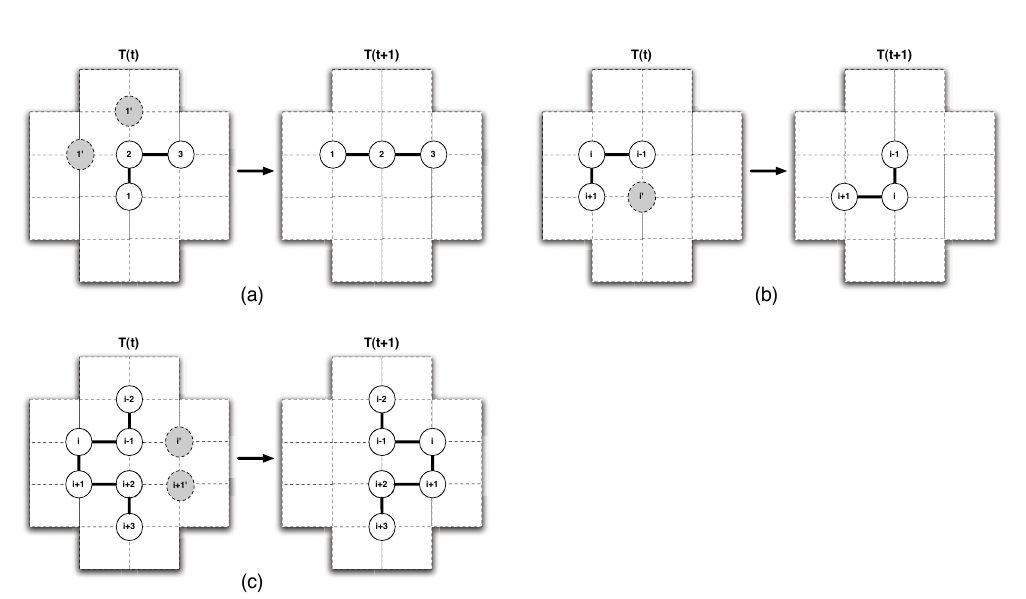
\includegraphics[width=400px]{./vshd.png}
\caption{\label{fig:moves}The 3 moves implemented : (a) end move (b) corner move (c) crankshaft move (figure from the article)}
\end{figure}




\section*{Results}
\label{sec:org2f98aec}
The results are a bit disappointing. The \emph{crankshaft} move implementation is buggy, moreover, the limited moveset allowed by the VSHD neighbourhood restricts the exploration to very close to the starting conformation. Moreover, the code is unoptimized as of yet, and is quite slow. The many copies involved with our implementation might be slowing the implementation of the procedure down.

Taken together, those two limitations limit the usefulness of our program : the conformation moves slowly without \emph{pull moves}, thus necessiting a lot of iteration our program can't compute fast enough. For instance, a run with 5 replicas, 50 global steps and 100 local steps of insulin (a 110 amino acid peptide) takes about 2 minutes, as we can see in the output Figure \ref{blc:out}(Appendices).

\section*{Discussion}
\label{sec:orge42e452}
Aside from the \emph{crankshaft} issue, which could be solved given more time, the salient issue of our code is optimization. The structure we used, with a class \texttt{Move} having itself a \texttt{Conformation} as an attribute, involves a lot of copy of similar data. The memory impact is obviously not an issue, but the copying itself takes some time. Using another implementation, such as not storing the \texttt{Conformation} as a lattice but as a chained list with position stored inside might have been a better choice, while storing moves as two lists of position and corresponding amino acid numbers might have been lighter. However, our current implementation would have been helped with a less high level language more suited to the task (for instance the choice of the authors of the original paper, C++). In particular, using pointers explicitly, with manual memory allocation, could have also clarified our implementation. Moreover, using a compiled language usually leads to much improved run times. On the other hand, using such a language  implies a more involved workflow, and might not have been possible given the deadline.

The other prominent issue of this project, is the approximations and mistakes of the original paper. On Figure 12, line 10 of the pseudo code, the \texttt{>} sign should actually be a \texttt{<} sign. This is actually the case in the source code, line 201 of \texttt{Conformation.cpp}. Moreover, the authors never mention the use of the Boltzmann constant in any of their energy calculations, for instance page 6. It does make sense, otherwise the equations are never balanced. But it is present in the source code, defined in \texttt{Const.h} line 98, and used in \texttt{Conformation.h} line 212. Without those two factors, the negative changes to conformations are very frequently accepted, leading to wrong results, even though the code might be otherwise correct (fortunately in our case, it wasn't).

Finally, we might speculate as to the effect of the \emph{pull moves}. Without them, the neighbourhood explored is very small, especially when starting with the protein as a line. It probably has a significant effect, especially as \emph{«any two valid sequence conformations on the 2D square lattice can be transformed into each other by a sequence of pull move»}, according to the authors. The use of a random walk as a starting point does not compensate for this fact.

\clearpage
\section*{Appendices}
\label{sec:orgd4ac2f7}
The main issues we had with this project are described in the discussion. We might add that the deadline seems a bit short for this kind of task, at least to obtain a satisfying, scientifically sound result. But that is probably too hopeful, given that it is initially a project conducted by three scientists during a way longer period of time. Also, as we are not very experienced with OOP, it is frequent that we fall into some implementation pitfall, that is quite long to struggle out of, and when we do we haven't learned much and have lost precious time.

Another issue I have with writing such lengthy and comlpex programs is the fact we haven't learn any debugging tools, and best practices. We used pdb, rather unsophisticatedly by writing
\begin{verbatim}
import pdb; pdb.set_trace()
\end{verbatim}

wherever we felt like the issue was. But building proper \emph{reprexes} should have been the focus. Especially, coding simple \textbf{non-random} starting conformation could have saved many headaches, but as we felt always pressed by time, we did not take the time to implement it. Additionally, the fact that the program is a Monte Carlo Markov Chain, debugging is hard because the issues, arising somewhat randomly, might not be very reproducible. So we should have built first non-random versions of our methods before implementing randomness.

\begin{verbatim}
[paulet@fedora Projet]$ time ./main.py 5 50 100 --file ./data/insulin.fasta
The starting conformation :
This conformation has 110 residues
The energy of this conformation is -5
 ---------------------------------
|                                 |
|                                 |
|                                 |
|                        PHP   P  |
|                        PPPH  P  |
|                         PPHPHH  |
|                      PPPHP  PP  |
|                      HPPH       |
|                       P         |
|                      HP         |
|                      H          |
|                     PH          |
|                     PH          |
|                      PP         |
|                       H         |
|   H       PH        PPP         |
|   HH      PH        PPHP        |
|    HHPHH PPH     PH    H        |
|        P HHHHPPP PH    PPHP     |
|        HHHH    HPPPPP PPP H     |
|         HH        HPHHH PPP     |
|                   HPP   PH      |
|                   HHH   PP      |
|                                 |
|                                 |
 ---------------------------------
The final conformation :
This conformation has 110 residues
The energy of this conformation is -7
 --------------------------------
|                                |
|                                |
|                                |
|                       PHPP  P  |
|                       PP H PP  |
|                     P PPPHPHH  |
|                     PPHHP P    |
|                     HP         |
|                    PPP         |
|                    PH          |
|                     H          |
|                     HP         |
|                     HP         |
|                     PPP        |
|   HH               H H         |
|    H                PP         |
|    HH    PPHHH       P         |
|     P    PPHHPHH    HP         |
|     HHPHH H  PPPPH  PHPPH      |
|      HH HHH  P  PPPP P  PH     |
|                  HPHHHPPPP     |
|                  HPP  PPPP     |
|                  HHH   H       |
|                                |
|                                |
 --------------------------------

real	1m59.378s
user	1m58.821s
sys	0m0.114s
\end{verbatim}
\captionof{figure}{\label{blc:out}A timed output of our program}

\begin{figure}[htbp]
\centering
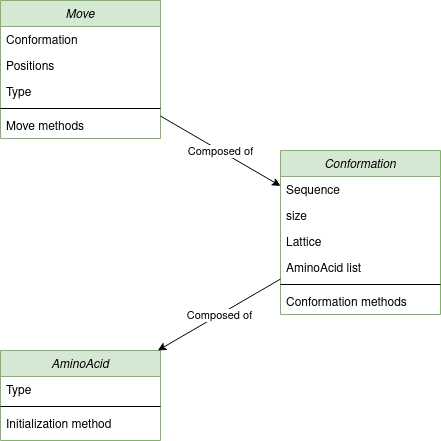
\includegraphics[width=300px]{./classes.png}
\caption{\label{fig:cls}The 3 classes implemented and their relation}
\end{figure}
\end{document}
